In der Messung werden für den Frequenzbereich von 6000 bis 9000 $\si{Hz}$ Rohrlängen von $\SI{75}{mm}$ bis $\SI{600}{mm}$ vermessen.
Bei bestimmten Frequenzen bildet sich eine Stehende Welle aus, das hat zur folge, dass die Schalwelle eine höhere Intensität hat.
In den folgenden 2 Abbildungen wird die Intensität gegen die Wellenlänge aufgetragen.
In der Abbildung \ref{fig.1} sind die Messwerte für die Rohrlängen : $\SI{75}{mm}, \SI{150}{mm}, \SI{225}{mm}, \SI{300}{mm}$ abbgebildet.
\begin{figure}[h!]
  \centering
  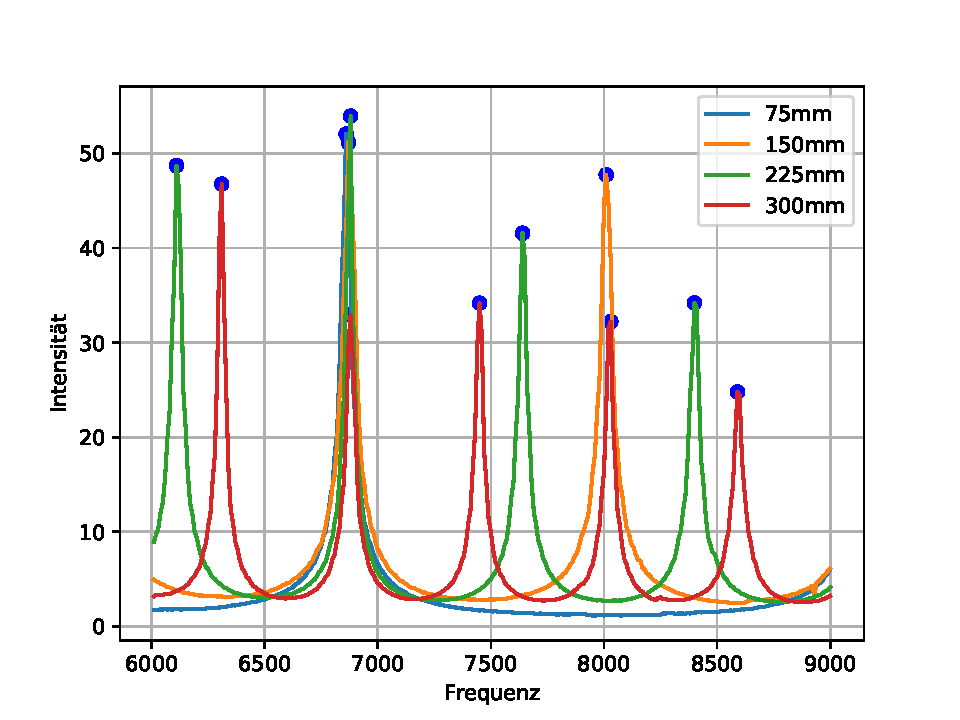
\includegraphics[width=\textwidth]{1234.pdf}
  \caption{Intensität der Sachalwelle im Bereich von 6000 bis 9000 $\si{Hz}$ für die Rohrlängen $\SI{75}{mm}, \SI{150}{mm}, \SI{225}{mm}, \SI{300}{mm}$}
  \label{fig.1}
\end{figure}
In der Abbildung \ref{fig.1} sind die Messwerte für die Rohrlängen : $\SI{375}{mm}, \SI{450}{mm}, \SI{525}{mm}, \SI{600}{mm}$ abbgebildet.
\begin{figure}[h!]
  \centering
  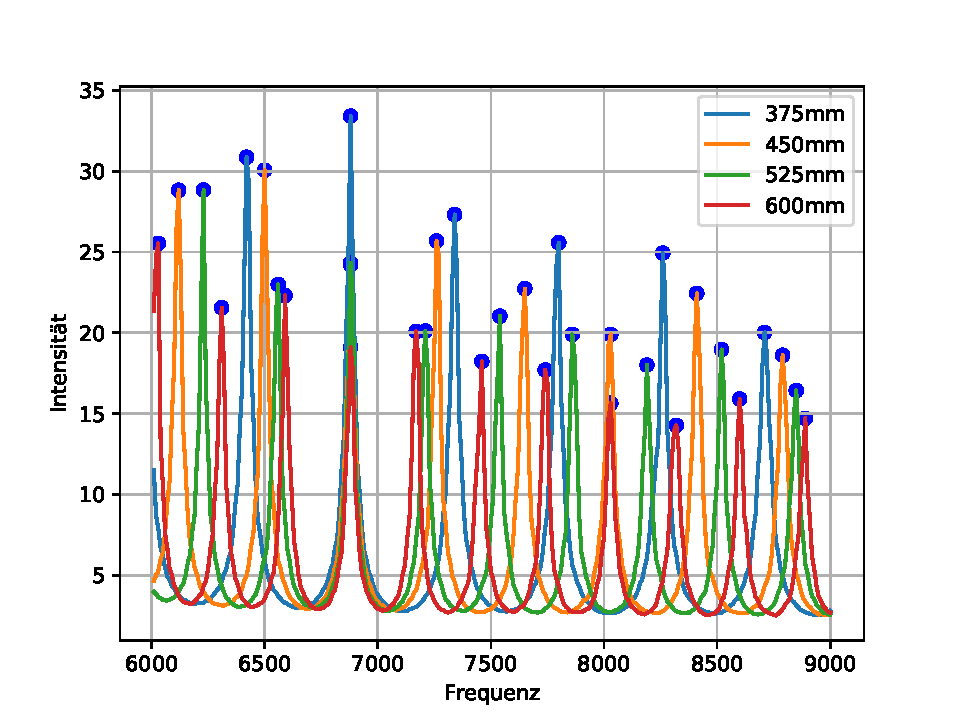
\includegraphics[width=\textwidth]{5678.pdf}
  \caption{Intensität der Sachalwelle im Bereich von 6000 bis 9000 $\si{Hz}$ für die Rohrlängen $\SI{375}{mm}, \SI{450}{mm}, \SI{525}{mm}, \SI{600}{mm}$}
  \label{fig.2}
\end{figure}
Die Intensitätsmaxima sind mit einem blauen Punkt gekenzeichnet.
Auffällig ist das sich für alle Rohrlängen Intensitätsmaximum an der Stelle von $\SI{6880}{Hz}$, das heißt, dass bei dieser Frequenz eine stehende Welle entsteht die eine Wellenlänge von $\lambda=\frac{1}{2n}d$ besitzt.
$d$ ist dabei die Länge des Rohres und n die Anzahl der Knotenpunkte.
Desweiteren ist auffällig, dass für eine Rohrlänge die Abstand zwichen zwei Maxima immer konstannt ist.

\subsection{Besimmung der Lichtgeschwindigkeit}
In den Graphen \ref{fig.2} und \ref{fig.2} werden die Resonanzfrequenzen einer jeden Messreihe von 1 bis n nummeriert und anschließend gegen die Frequenz aufgetragen.
Die Resonazfrequenzabstände sind konstant für eine Messreihe daher ergeben sich Geraden der Form: $y=ax+b$ welche an die Messwerte gefittet werden.
In der Abb. \ref{fig.linearfit} sind die Messwerte mit den Fitfunktionen abgebildet.
%Für die Fitparameter ergeben sich folgende Werte.
%\begin{align*}
%  a &= 286.54545455 \pm 0.37848474\\
%  b &= 5737.09090907 \pm 2.56700835
%\end{align*}
Mit Hilfe der Steigung $a$ kann als die Schallgeschwindigkeit $c$ berechnet werden.
\begin{align*}
  c = a\cdot2d
\end{align*}
Für die Schallgeschwindigkeit ergeben sich so Werte von:
\begin{align*}
c&=342.0\\
c&=343.3\\
c&=342.6\\
c&=343.9\\
c&=343.5\\
c&=343.8\\
\end{align*}
%###########Bild##########
%\begin{figure}[h!]
%  \centering
%  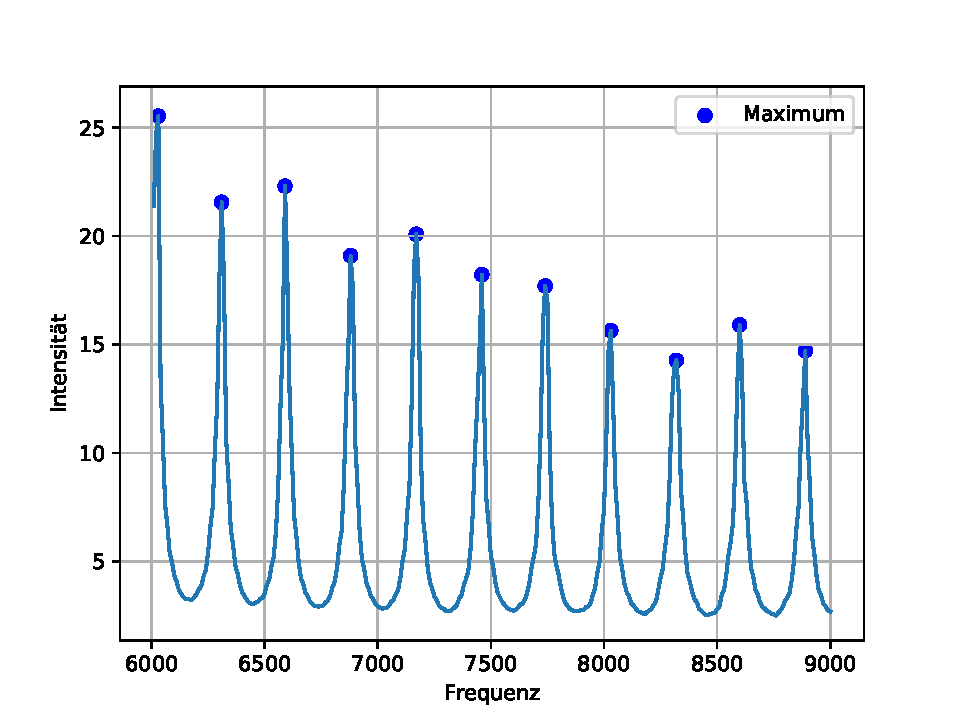
\includegraphics[width=\textwidth]{A1L8x75mmF6000-9000S10.pdf}
%  \caption{Messung eines $\SI{0.6}{m}$ Rohres für den Frequenzbereich von 6000 bis 9000 Hz}
%  \label{fig.frequenz/rohrlänge}
%\end{figure}
\begin{figure}[h!]
  \centering
  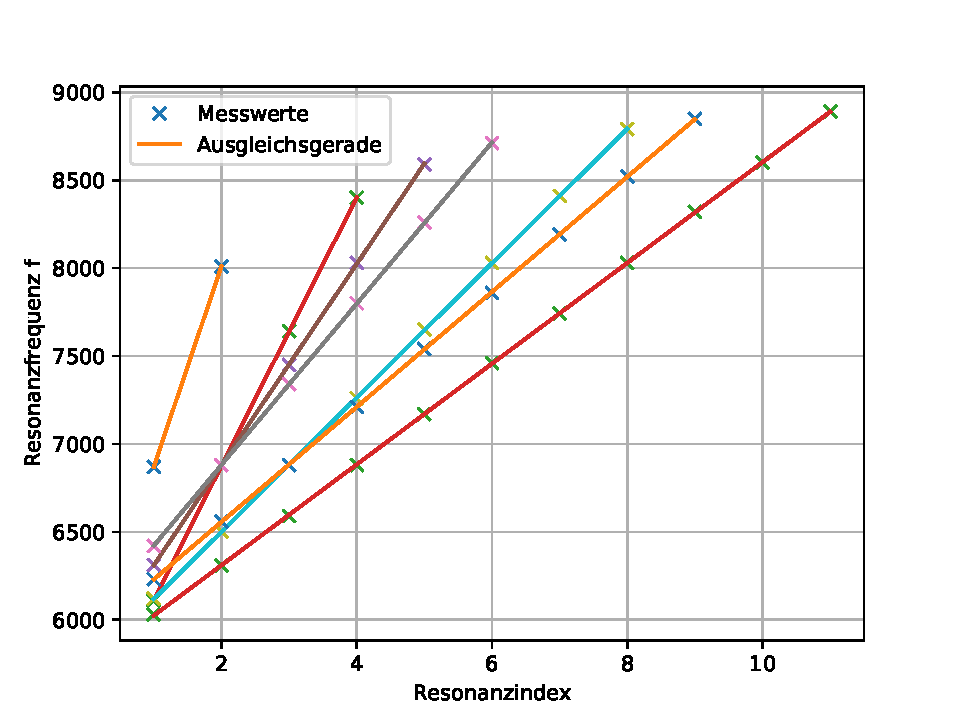
\includegraphics[width=\textwidth]{linearfit.pdf}
  \caption{Die Intensitätsmaxima werden nummerriert und die Nummer gegen die Frequenz aufgetragen.}
  \label{fig.linearfit}
\end{figure}
%#########
\FloatBarrier
Die Schallgeschwindigkeit kann auch mit Hilfe einer anderen Methode bestimmt werden.
dazu betrachten wir ein Rohr der Länge 75mm für die Frequenzen von 6000 bis 9000 $\si{Hz}$.
Da die Rohrlänge $d$ ein vielfaches $n$ der halben Wellenlänge $\lambda$ ist gilt:
\begin{align*}
  \lambda = \frac{2d}{n}
\end{align*}
Die Schallgeschwindigkeit ist gegeben durch:$c=f \cdot \lambda$
Daraus ergiebt sich :
\begin{align}
  n&=1  c&=\SI{1032}{\frac{m}{s}}\\
  n&=2  c&=\SI{516}{\frac{m}{s}}\\
  n&=3  c&=\SI{344}{\frac{m}{s}}\\
  \label{eqn.schall}
  n&=4  c&=\SI{258}{\frac{m}{s}}
\end{align}
Die Freqenz ist dabei gegeben als $\SI{6880}{\frac{m}{s}}$.
Diese Freqenz ist die einzige Frequenz im Frequenzbereich welche bei allen Vielfachen der Rohrlänge von $\SI{75}{mm}$ vertreten ist,
zusehen ist dies in den Abb. \ref{fig.1234} und \ref{fig.5678}.
Den Ergebnissen aus \ref{eqn.schall} ist zu entnehmen, dass die Wellenlänge bei $\frac{3}{2}\lambda$ liegt, da die dazugehörige Schallgeschwindigkeit von $\SI{344}{\frac{m}{s}}$ gut zum Litteraturwert??? von $\SI{343.2}{\frac{m}{s}}$ passt.

\FloatBarrier
Desweiteren soll die Schallgeschwindigkeit Mithilfe des Verhätnisses von Frequenzübergang zu Rohrlänge bestimmt werden.
Dieser Zusammenhang ist in Abb. \ref{fig.1/x} dargestellt.
An die Messwerte wird eine Funktion der Form $a\cdot\frac{1}{x}+b$ gefittet.
Für a und b ergegben sich die Werte:
\begin{align*}
  a&=1.68692913\cdot10^5\pm253.97695158\\
  b&=8.56657992\pm1.99530368\\
\end{align*}
%################Bild#####################
\begin{figure}[h!]
  \centering
  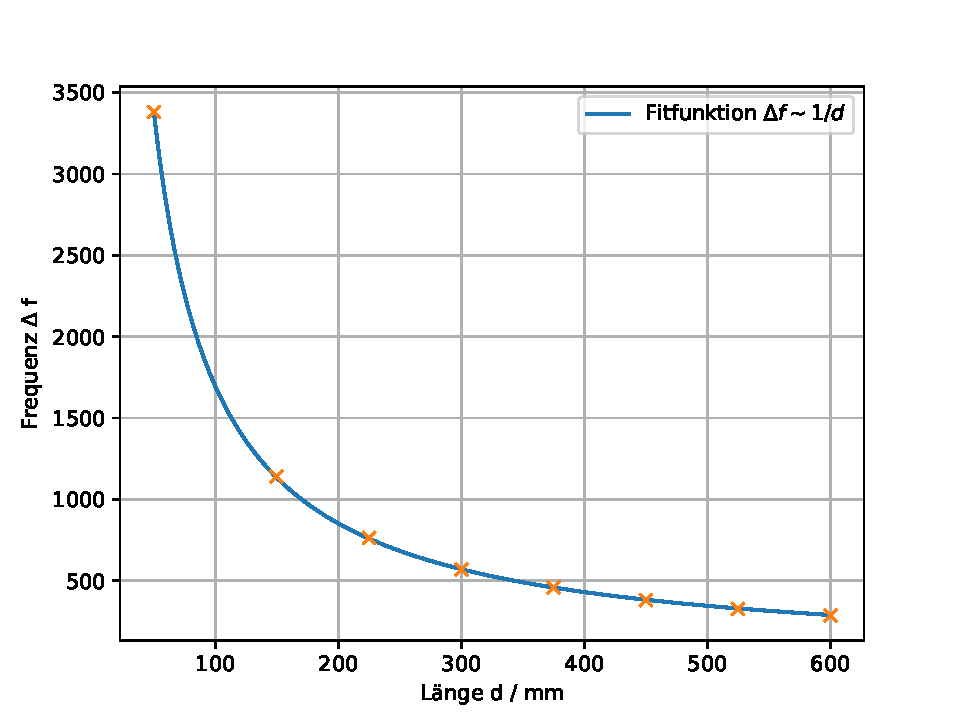
\includegraphics[width=\textwidth]{geschi.pdf}
  \caption{Der Abstand der Frequenzen wird gegen die Rohrlänge Aufgretragen.}
  \label{fig.1/x}
\end{figure}

\subsection{Aufgabe 2?}
bestimmung von k
\begin{align*}
  k= \frac{2\pi}{\lambda}
\end{align*}
w
\begin{align*}
  \omega=2\pi f
\end{align*}
\begin{align*}
  \omega_k=k\lambda f
\end{align*}
Linear nochmal mit wk anstat freqenz oder anders
